\section{DP優化}
    \subsection{前言}
    這個單元我會提及一些優化技巧,但是因為有許多優化我是不清楚的,
    所以我可以提供的也很有限。

    \subsection{滾動陣列}
    在上一個單元我們有提到背包問題,其中,我們的空間複雜度為
    $O(nW)$,再有一些競賽上,我們可能不允許有那麼多的記憶體空間,
    這時候我們可以觀察遞迴式,並發現在背包問題當中,
    我們每一次都只會用到第$i$項,所以我們會需要的只有兩行陣列。

    實作上,我們可以藉由位元運算來達成。當然也可以用\%,不過位元運算
    看起來帥,而且還有比較小的常數。

\begin{lstlisting}[caption=01背包]
ll dp[2][100010],v[105],w[105];

int main(){
    // input
    for(int i=1;i<=n;i++){
        for(int j=1;j<=W;j++){
            if(w[i]>j){
                dp[i&1][j]=dp[i&1^1][j];
            }else{
                dp[i&1][j]=max(dp[i&1^1][j],dp[i&1^1][j-w[i]]+v[i]);
            }
        }
    }
    cout<<dp[n&1][W];
}
\end{lstlisting}

    \subsection{狀態壓縮}
    讓我們看看以下問題。

    \example TIOJ 1014  打地鼠

    \textbf{題目敘述}

    隨著時間的腳步前進,打地鼠遊戲也不斷的翻新,最新一代的打地鼠遊戲不只測試你的反應能力,
    同時也考驗著你的體力和智力。地鼠基地是一個長型的基座,基座上每隔一公尺就會有一個地鼠洞,
    由左至右編號為 $1$ 到 $n$。玩家站在這個基地的最左邊,與第一個地鼠洞相距1公尺;
    拿著一根鎚子,準備開始這個遊戲。編號為 $i$ 的地鼠洞每 $T_i$
    秒地鼠會出現一次。被打的地鼠不再出現,只要將所有地鼠打完,就結束遊戲,
    並且紀錄從開始到結束遊戲的秒數,越快越好。現在問題來了,
    負責製造這個地鼠基地的遊戲廠商想要知道結束遊戲所需的最少秒數,於是拜託你幫忙寫個程式來解決它。

    假定玩家們的體力很好,隨時以每秒1公尺的速度移動,並且不受移動方向改變的影響,打地鼠所花的時間也可以忽略不計。

    \textbf{輸入說明}

    第一行有一個數字$n, n \le 16$,代表地鼠洞的數量。第二行有 
    $n$個數字。所有數字皆不大於$10^8$。

    \textbf{輸出說明}

    請輸出結束遊戲所需的最少秒數$S$。

    \textbf{範例測試}

    \begin{tabular}{|m{7cm}|m{7cm}|}
        \hline
        範例輸入 1 & 範例輸出 1 \\
        \hline
        \verb|3| & \verb|5| \\
        \verb|3 2 5| & \\
        \hline
    \end{tabular}

    \textbf{想法}

    其實這算是另外一種DP的類型,因此,我會從狀態的定義開始講起。
    你應該有發現這題的n超小,而TIOJ基本上沒有很水的測資範圍。所以
    根據經驗,我們需要能夠判斷這是一個$O(2^n)$以上,$O(n!)$以下的
    題目。

    首先,請考慮n很小的情況,例如$n=3$,我們將會需要這樣定義狀態。

    $$dp[m][i_1][i_2][i_3], i_1,i_2,i_3 \in \{0, 1\} := 打完地鼠停在位置m所需要的最短時間$$

    其中,$i_1,i_2,i_3$表示第1,2,3之地鼠有沒有被打過,0表示沒有,1表示有。

    然而,我們最終要解決的問題對多是16之地鼠,但是我們不會想要開17維陣列。
    所以我們可以將陣列的位址壓縮在一個變數裡面,這樣的技巧不只會在DP用到,
    不過我們有點晚才講(將來也有可能會編到第三章)。

    實際上要怎麼做呢?我們知道,$i_1,i_2, \cdots , i_n$都只有0或1。
    那我們何不使用int來存。因為int有32個bit,每一個bit都可以存0或1。

    $$dp[m][a] := 將所有i_k壓所成狀態a$$
    除此之外,我們還需要實作一個函式GetWaitTime,
    這個函式將會告訴從狀態a轉移到狀態b需要花多久。

    那轉移式呢?我們可以從m以外的所有點走過來。

    $$
    \begin{cases}
        dp[0][0]=1 \\
        dp[m][a]=\min (dp[k][a-2^{m}]+GetWaitTime(a,a-2^m,dp[k][a-2^m])) \\ 
        1 \le k \le n, \; 如果你從k轉移到m
    \end{cases}
    $$

    \textbf{實作}

\begin{lstlisting}[caption={TIOJ 1014題解}]
#define int ll
using ll=long long;
const ll INF=0x3f3f3f3f3f3f3f3f;

// 實際上應該是 1<<16 就夠用了
int a[20],dp[20][1<<19];

int GetWaitTime(int to,int from,int timeNow){
    int ret=abs(from-to);//time to walk to there
    timeNow+=ret;//time now when walk to target

    //if timeNow=10, a[to]=3 then player should wait 2sec
    if(timeNow%a[to]!=0)
        ret+=a[to]-(timeNow%a[to]);

    return ret;
}

int32_t main(){
    ios::sync_with_stdio(0);cin.tie(0);
    
    int n;
    cin>>n;

    for(int i=0;i<n;++i){
        cin>>a[i];
    }

    for(int i=0;i<20;++i){
        fill(dp[i],dp[i]+(1<<19),INF);
    }

    dp[0][0]=1;

    // 藉由位元運算表達此過程,建議複習位元運算。
    for(int i=1;i<(1<<n);++i){
        for(int j=0;j<n;++j){
            if(!(i&(1<<j))) continue;
            for(int k=0;k<n;++k){
                dp[j][i]=min(
                    dp[j][i],
                    dp[k][i-(1<<j)]+GetWaitTime(j,k,dp[k][i-(1<<j)])
                );
            }
        }
    }

    int ans=INF;

    for(int i=0;i<n;++i){
        ans=min(ans,dp[i][(1<<n)-1]);
    }

    cout<<ans;
}
\end{lstlisting}

    \subsection{資料結構優化}
    顧名思義,就是利用資料結構,幫助加速轉移式。
    通常用於轉移複雜度$O(n)$或更高的問題。使用BIT,線段樹等資料結構。

    \example 111宜中校內賽 F 波動的麥穗

    \textbf{題目敘述}

    傳說蘇格拉底曾經帶領幾個弟子來到一個麥穗田邊,請他們去摘下一個最高最好的麥穗。
    不過他們必須頭也不回地沿著直線前進,且只有一次的摘取機會。
    這個故事逐漸演變成數學裡的最優停止問題(Optimal Stopping Problem),並且找到了最佳解 —— $37\%$ 法則。
    也就是記住前 $37\%$ 中最高最好的麥穗,接著在後 $63\%$ 裡頭遇到的第一個更好的麥穗即是最佳選擇。

    某晚小晨在睡夢中偶遇了蘇格拉底,最近因為股市起起落落而心情大受影響的小晨,忍不住跟蘇格拉底抱怨一番。
    為了鼓勵小晨繼續努力前進,蘇格拉底又講述了一個麥穗的故事。
    不同於先前的版本,這次蘇格拉底希望小晨去尋找一些高度波動的麥穗,就好像那高高低低的股價一般。
    蘇格拉底說到

    「小晨啊,你看看眼前的 $N$ 個麥穗,每個都有不同的高度 $h_i$ 跟價值 $v_i$。
    不如你就去尋找一些麥穗,使得你依序選定的這些麥穗高度是波動的,且價值總和最高。
    相信這一定會對你的人生有所幫助吶!」

    更確切地說,若 $h_1, h_2, \cdots, h_k$ 依序是小晨選定的麥穗高度,則這些高度必須滿足波動形式:
    $$
        \left(h_{j-1} < h_j > h_{j+1}\right) \vee 
        \left(h_{j-1} > h_j < h_{j+1}\right)
        ,\quad \forall j \in [2, k-1]
    $$
    也就是這些選定的麥穗一字排開的話,高度會呈現一高一低的鋸齒狀。

    小晨醒來後,急忙拿著這 $N$ 筆麥穗的資料翻來覆去,嘗試尋找最佳的選擇。
    然而由於麥穗實在是太多了,小晨怎麼樣也無法好好確認所有的可能性。
    請你幫助小晨,找到最佳選擇下,他能夠拿到多少價值總和的麥穗,讓他的人生可以稍微減少一點悲慘。

    \textbf{輸入說明}

    第一行包含一個正整數 $N$,代表麥穗的數量。

    接下來 $N$ 行,每行有二個整數 $h_i, v_i$,分別代表第 $i$ 個麥穗的高度與價值。

    各變數範圍限制如下:
    \begin{itemize}
        \item $1 \le N \le 2\times 10^5$
        \item $-10^9 \le h_i, v_i \le 10^9$
    \end{itemize}

    \textbf{輸出說明}

    請輸出一個整數,代表最高可能的價值總和。

    \textbf{範例測試}

    \begin{tabular}{|m{7cm}|m{7cm}|}
        \hline
        範例輸入 1 & 範例輸出 1 \\
        \hline
        \parbox[t]{7cm} % sample 1
        { \tt
        % input
        10 \\
        2 7 \\
        3 5 \\
        6 1 \\
        5 3 \\
        7 2 \\
        1 8 \\
        3 9 \\
        6 2 \\
        4 1 \\
        5 3 \\
        } &
        \parbox[t]{7cm}
        { \tt
        %output
        30 \\
        } \\
        \hline
    \end{tabular}

    \begin{figure}[!htbp]
        \centering
        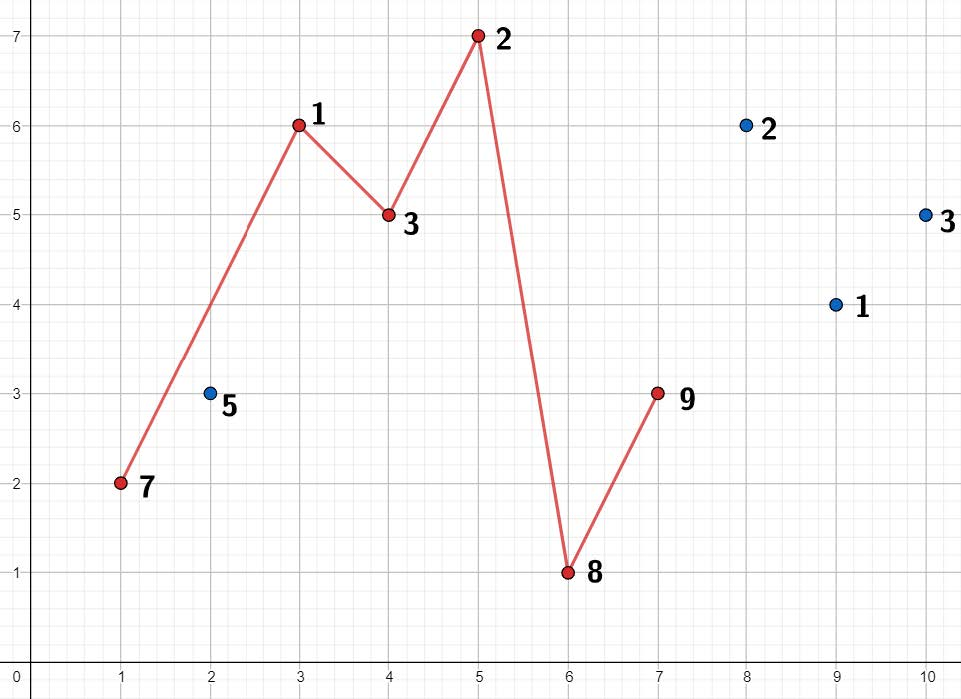
\includegraphics[width=0.8\textwidth]{../Images/DP4.jpg}
    \end{figure}

    \textbf{想法}

    如果你DP有學好的話,我們可以很輕易的定義出這樣的狀態。

    $$\begin{cases}
        dp[0][n] := 以第n個麥穗為結尾時,
        且前一個選的麥穗比他高的最大價值\\
        dp[1][n] := 以第n個麥穗為結尾時,
        且前一個選的麥穗比他低的最大價值
    \end{cases}$$

    並列出這樣的轉移式。

    $$\begin{cases}
        dp[0][n] := \max(dp[1][i])+v[n], \; for \; h[i]>h[n]\\
        dp[1][n] := \max(dp[0][i])+v[n], \; for \; h[i]<h[n] \\
        1 \le i < n
    \end{cases}$$

    我們可以發現,這樣會需要$O(n)$的複雜度進行轉移,所以總時間複雜度會是$O(n^2)$。
    這樣沒有辦法拿到全部的分數。所以,我們需要優化找有條件的最大值的時間。

    我們可以使用值域線段樹或Treap。當時我使用的是Treap,其時間複雜度為$O(\log n)$,
    以題目測資範圍而言是$\log(10^5)$,但是其實這一題用值域線段樹也會過,雖然複雜度比較高,
    為$O(\log C)$,是$\log(2 \times 10^9)$。不過要注意Treap的常數比較大
    (而且code比較長)。

    我們的Treap以h[i]為key,裡面存放與維護max dp值,查詢時就切$key<h[i]$
    以及$key>h[i]$下來就可以了。

    答案會是整個dp表格中的最大值。

    \subsection{其他資源}
    
    \url{https://hackmd.io/@Ccucumber12/Bk6lLyuxF#/}

    \begin{figure}[!htbp]
        \centering
        
\includegraphics[width=0.2\textwidth]{../Images/DP5.png}
    \end{figure}

    \url{https://cp-algorithms.com/dynamic_programming/divide-and-conquer-dp.html}

    \begin{figure}[!htbp]
        \centering
        
\includegraphics[width=0.2\textwidth]{../Images/DP6.png}
    \end{figure}

    \subsection{範例與練習}

    \begin{tip}
        接下來的問題不一定需要DP優化。
    \end{tip}

    \problem 110 年林燈 APCS 選手班 暑期賽 E 瘋搶口罩
    
    \textbf{題目敘述}

    疫情肆虐,全球封城。武漢肺炎迅速傳播,口罩成了民眾日常的必需品。
    膽小的YL 想買一盒又一盒的口罩塞滿家裡,好讓日子更安心,
    出門不擔心。在 YL 的居住城鎮裡共有$N$間販賣口罩的藥局,
    其中第 $i$ 間藥局一盒口罩要價 $p_i$ 元,
    能提供 $s_i$ 單位的安心度。為了避免民眾囤積口罩,
    造成物資短缺,DCD 規定在同一間藥局只能購買一盒口罩。
    但是擁有高超交際手腕的 YL,能夠透過一些技術性的操作打破此限制。
    在第 $i$ 間藥局,他只要包 $r_i$ 元的紅包給藥師,
    就能在該藥局購買任意數量的口罩。然而他也不能無限制得亂來,
    否則很有可能會被查水表,鋃鐺入獄。為了避免過於招搖,
    YL 最多只能偷塞 $K$ 個紅包。今日一早,YL 去銀行提領了 $M$ 元,
    打算全部拿來購買口罩。請問在有效運用經費的情況下,
    YL 最多能夠獲得多少安心度總和?

    \textbf{輸入說明}

    第一行包含三個整數 $N$、$M$ 和 $K$。

    接下來的 $N$ 行,每行包含三個整數 $p_i$、$s_i$ 和 $r_i$。

    $1 \le N \le 100$,$0 \le K \le N$,$1 \le M \le 5000$
    
    $1 \le p_i \le 5000$,$0 \le r_i \le 5000$,$1 \le s_i \le 10^6$

    所有輸入數字皆為整數

    \textbf{輸出說明}

    輸出 YL 最多能夠獲得多少安心度總和。

    \textbf{範例測試}

    \begin{tabular}{|m{7cm}|m{7cm}|}
        \hline
        範例輸入 1 & 範例輸出 1 \\
        \hline
        \verb|4 20 1| & \verb|26| \\
        \verb|3 4 2| & \\
        \verb|2 5 10| & \\
        \verb|7 9 3| & \\
        \verb|4 2 1| & \\
        \hline
    \end{tabular}

    \problem TIOJ 1019 E.Jumping Up

    \textbf{題目敘述}

    
    沒錯,這個問題就跟兔子跳鈴鐺有關。

    有一顆超級大番茄(因為頭很大,所以簡稱大頭蕃)非常喜歡玩這個遊戲,
    可是每次滑鼠都要左移、右移,一不小心就會掉下去,又得從頭開始了,
    挺累人的說。遊戲中的兔子從跳上第一個鈴鐺開始,每次跳起來的最大高度只夠這隻兔子跳到下一個、
    或是第兩個鈴鐺上,而且鈴鐺一旦被踩過就會消失(然後兔子跳了起來)。
    現在給你n個鈴鐺的水平位置,請你告訴大頭蕃從第一個鈴鐺開始一路跳到第 n個鈴鐺所需的最小移動水平距離總和為何?
    (我們在這個題目中假設可以踩的飛鳥不曾出現,而且不必每個鈴鐺都踩過。)

    p.s.以上故事純屬虛構,但是測資並非虛構(不好笑…)

    \textbf{輸入說明}

    輸入檔的第一列有一個正整數$T(T \le 1000)$,代表接下來的測試資料總數。
    
    接下來的每一列都是一組測試資料,首先會有一個正整數n,
    接下來依序會有第一個鈴鐺到第n個鈴鐺相對於螢幕正中央的水平位移$d_1,d_2, \cdots , d_n$。
    其中任意的$d_i, 1 \le i \le n$都可以用有號的32-bit integer儲存。

    \textbf{輸出說明}

    對於每一筆測試資料,請輸出一個正整數代表從第一個鈴鐺跳上第N個鈴鐺所需要的最小水平距離總長。

    \textbf{範例測試}

    \begin{tabular}{|m{7cm}|m{7cm}|}
        \hline
        範例輸入 1 & 範例輸出 1 \\
        \hline
        \verb|1| & \verb|8| \\
        \verb|9 1 2 3 4 5 6 7 8 9| & \\
        \hline
    \end{tabular}

    \begin{tip}
        AtCoder DPC A Frog1
    \end{tip}

    \problem TIOJ 1288 D. [IOI 1994] 三角旅行

    \textbf{題目敘述}

    一個有數字構成的正三角形。現在請求出從最頂端走到最底端 最大的和是多少。

    每個點只能往左下或右下走,底層的點不能再往下走。

    三角形的高度介於 1 到 100 之間。
    三角形上的數字都介於 0 到 99 之間。

    \textbf{輸入說明}

    第一個是數字 n 代表三角形高度。聰明的你知道接下來是怎樣的格式。

    \textbf{輸出說明}

    輸出一個貌似解答的數字。

    \textbf{範例測試}

    \begin{tabular}{|m{7cm}|m{7cm}|}
        \hline
        範例輸入 1 & 範例輸出 1 \\
        \hline
        \verb|5| & \verb|30| \\
        \verb|7| & \\
        \verb|3 8| & \\
        \verb|8 1 0| & \\
        \verb|2 7 4 4| & \\
        \verb|4 5 2 6 5| & \\
        \hline
    \end{tabular}

    \problem TIOJ 1291 N 箱 M 球

    \textbf{題目敘述}

    n個相同的箱子要放入m個不同的球,問有幾種放法。(對$10^6$取餘)

    n=m=0 代表測試資料結束。

    \textbf{範例測試}

    \begin{tabular}{|m{7cm}|m{7cm}|}
        \hline
        範例輸入 1 & 範例輸出 1 \\
        \hline
        \verb|26 11| & \verb|678570| \\
        \verb|21 45| & \verb|517677| \\
        \verb|0 0| & \\
        \hline
    \end{tabular}

    \begin{tip}
        模逆元可以用嗎?
    \end{tip}

    \problem CF 698A Vacations

    \textbf{題目敘述}

    $Vasya$ 有 $n$ 天的假期!所以他決定提升自己的$IT$技能並進行運動。$Vasya$ 對於每一天的假期都知道以下信息:健身房是否開放以及當天是否在網路上舉辦比賽。對於第 $i$ 天,有四種情況:

    在這一天,健身房關閉且沒有舉辦比賽;
    在這一天,健身房關閉且舉辦了比賽;
    在這一天,健身房開放且沒有舉辦比賽;
    在這一天,健身房開放且舉辦了比賽。

    在每一天,$Vasya$ 可以選擇休息,參加比賽(如果當天有比賽),或進行運動(如果健身房當天開放)。

    找出 $Vasya$ 至少需要休息的天數(意味著他不能同時進行運動和參加比賽)。$Vasya$ 唯一的限制是:他不想在連續兩天做相同的活動,也就是說他不會在連續兩天進行運動,或連續兩天參加比賽。

    \textbf{輸入說明}

    第一行包含一個正整數 $n$ $(1 \le n \le 100)$ — $Vasya$ 的假期天數。

    第二行包含由空格分隔的整數序列 $a_1, a_2, ..., a_n$ $(0 \le a_i \le 3)$,其中:

    $a_i = 0$,表示在第 $i$ 天的假期中,健身房關閉且沒有舉辦比賽;
    
    $a_i = 1$,表示在第 $i$ 天的假期中,健身房關閉且舉辦了比賽;
    
    $a_i = 2$,表示在第 $i$ 天的假期中,健身房開放且沒有舉辦比賽;
    
    $a_i = 3$,表示在第 $i$ 天的假期中,健身房開放且舉辦了比賽。

    \textbf{輸出說明}

    輸出 $Vasya$ 至少需要休息的天數。請記住 $Vasya$ 拒絕在連續兩天進行運動,
    在連續兩天參加比賽。

    \textbf{範例測試}

    \begin{tabular}{|m{7cm}|m{7cm}|}
        \hline
        範例輸入 1 & 範例輸出 1 \\
        \hline
        \verb|4| & \verb|2| \\
        \verb|1 3 2 0| & \\
        \hline
    \end{tabular}

    \problem CF 1195 C Basketball

    \textbf{題目敘述}

    終於,一個籃球場在SIS開幕了,因此Demid決定舉行籃球訓練課程。有2n名學生參加了Demid的訓練課程,他將他們分成兩排,每排都有n個學生(每排有恰好n個學生)。學生在每排中從左到右按順序編號從1到n。

    現在Demid想要選擇一支籃球隊。他會按照從左到右的順序選擇球員,並且每個被選擇的球員的索引(不包括第一個選擇的球員)必須嚴格大於先前選擇的球員的索引。為了避免偏袒某一排,Demid選擇學生的方式是不允許連續選擇同一排的學生。第一個球員可以從所有2n名學生中選擇(沒有額外的限制),並且一支隊伍可以包含任意數量的球員。

    \begin{figure}[!htbp]
        \centering
        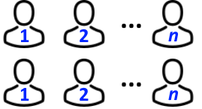
\includegraphics[width=0.4\textwidth]{../Images/CF1195.png}
    \end{figure}

    Demid認為為了組成一支完美的隊伍,他應該以使得所選球員的總身高盡可能最大的方式進行選擇。幫助Demid找到他可以選擇的隊伍的最大可能總身高。

    \textbf{輸入說明}

    輸入的第一行包含一個正整數$n(1 \le n \le 10^5)$——每排的學生數量。

    輸入的第二行包含n個整數$h_{1,1}, h_{1,2}, \cdots, h_{1,n}(1 \le h_{1,i} \le 10^9)$,其中$h_{1,i}$表示第一排第i個學生的身高。

    輸入的第三行包含n個整數$h_{2,1}, h_{2,2}, \cdots, h_{2,n}(1 \le h_{2,i} \le 10^9)$,其中$h_{2,i}$表示第二排第i個學生的身高。

    \textbf{輸出說明}

    輸出一個整數——Demid可以選擇的隊伍的最大可能總身高。

    \textbf{範例測試}

    \begin{tabular}{|m{7cm}|m{7cm}|}
        \hline
        範例輸入 1 & 範例輸出 1 \\
        \hline
        \verb|5| & \verb|29| \\
        \verb|9 3 5 7 3| & \\
        \verb|5 8 1 4 5| & \\
        \hline
    \end{tabular}

    \problem CF 474 D Flowers

    \textbf{題目敘述}

    我們看到土撥鼠為鼴鼠的午餐準備的小遊戲。現在輪到土撥鼠晚餐時間了,眾所周知,土撥鼠吃花朵。在每頓晚餐中,他會吃一些紅色和白色的花朵。因此,一頓晚餐可以表示為一系列的花朵,其中有些是白色的,有些是紅色的。

    但是,為了讓晚餐美味,有一個規則:土撥鼠只想以大小為k的組合吃白色花朵。

    現在土撥鼠想知道他可以以多少種方式吃掉a到b朵花。由於方式的數量可能非常大,請將其按照$1000000007$($10^9+7$)取模後輸出。

    \textbf{輸入說明}

    輸入包含多個測試案例。

    第一行包含兩個整數$t$和$k$ ($1\leq t, k\leq 105$),其中$t$表示測試案例的數量。

    接下來的$t$行包含兩個整數$ai$和$bi$ ($1\leq ai\leq bi\leq 105$),描述第$i$個測試案例。

    \textbf{輸出說明}

    將結果輸出到標準輸出,共$t$行。第$i$行應該包含土撥鼠在晚餐時可以吃掉$ai$到$bi$朵花的方式數,取模於$1000000007$ ($10^9+7$)。

    \textbf{範例測試}

    \begin{tabular}{|m{7cm}|m{7cm}|}
        \hline
        範例輸入 1 & 範例輸出 1 \\
        \hline
        \verb|5| & \verb|29| \\
        \verb|9 3 5 7 3| & \\
        \verb|5 8 1 4 5| & \\
        \hline
    \end{tabular}

    \problem CF 4D Mysterious Present

    \textbf{題目敘述}

    Peter決定向他在澳大利亞的朋友送上生日快樂的祝福,並寄去一張賀卡。為了讓他的禮物更加神秘,他決定做一條鏈子。鏈子是由信封組成的序列 $A={a_1, a_2, \ldots, a_n}$,其中第 $i$ 個信封的寬度和高度都嚴格大於前一個信封的寬度和高度。鏈子的大小是鏈子中信封的數量。

    Peter希望從他擁有的信封中製作出最大尺寸的鏈子,該鏈子應該能夠容納一張卡片。如果卡片的寬度和高度都小於鏈子中最小信封的寬度和高度,則卡片可以放入鏈子中。禁止旋轉卡片和信封。

    Peter擁有非常多的信封,但時間非常有限,這個艱鉅的任務交給了你。

    \textbf{輸入說明}

    第一行包含兩個整數 $n$ 和 $w$、$h$ $(1\leq n\leq 5000, 1\leq w, h\leq 10^6)$ —— Peter擁有的信封數量,以及卡片的寬度和高度。接下來的 $n$ 行中,每行包含兩個整數 $w_i$ 和 $h_i$ $(1\leq w_i, h_i\leq 10^6)$ —— 第 $i$ 個信封的寬度和高度。

    \textbf{輸出說明}

    在第一行輸出最大鏈子的大小。在第二行輸出形成所需鏈子的信封編號(以空格分隔),從最小信封的編號開始。請注意,卡片應該放入最小的信封中。如果最大尺寸的鏈子不唯一,則可以輸出其中任意一個答案。

    \textbf{範例測試}

    \begin{tabular}{|m{7cm}|m{7cm}|}
        \hline
        範例輸入 1 & 範例輸出 1 \\
        \hline
        \verb|2 1 1| & \verb|1| \\
        \verb|2 2| & \verb|1| \\
        \verb|2 2| & \\
        \hline
    \end{tabular}
    
    \problem 洛谷 P3959 [NOIP2017 提高組] 寶藏

    \textbf{題目敘述}

    參與考古挖掘的小明得到了一份藏寶圖,藏寶圖上標出了 $n$ 個深埋在地下的寶藏屋, 也給出了這 $n$ 個寶藏屋之間可供開發的 $m$ 條道路和它們的長度。

    小明決心親自前往挖掘所有寶藏屋中的寶藏。但是,每個寶藏屋距離地面都很遠,也就是說,從地面打通一條到某個寶藏屋的道路是很困難的,而開發寶藏屋之間的道路則相對容易很多。

    小明的決心感動了考古挖掘的贊助商,贊助商決定免費贊助他打通一條從地面到某個寶藏屋的通道,通往哪個寶藏屋則由小明來決定。

    在此基礎上,小明還需要考慮如何開鑿寶藏屋之間的道路。已經開鑿出的道路可以任意通行不消耗代價。每開鑿出一條新道路,小明就會與考古隊一起挖掘出由該條道路所能到達的寶藏屋的寶藏。另外,小明不想開發無用道路,即兩個已經被挖掘過的寶藏屋之間的道路無需再開發。

    新開發一條道路的代價是 $\mathrm{L} \times \mathrm{K}$。其中 $L$ 代表這條道路的長度,$K$ 代表從贊助商幫你打通的寶藏屋到這條道路起點的寶藏屋所經過的寶藏屋的數量(包括贊助商幫你打通的寶藏屋和這條道路起點的寶藏屋)。

    請你編寫程式為小明選定由贊助商打通的寶藏屋和之後開鑿的道路,使得工程總代價最小,並輸出這個最小值。

    \textbf{輸入說明}

    第一行兩個用空格分離的正整數 $n,m$,代表寶藏屋的個數和道路數。

    接下來 $m$ 行,每行三個用空格分離的正整數,分別是由一條道路連接的兩個寶藏屋的編號(編號為 $1-n$),和這條道路的長度 $v$。

    $1 \le n \le 12$,$0 \le m \le 10^3$,$v \le 5\times 10^5$

    \textbf{輸出說明}

    一個正整數,表示最小的總代價。

    \textbf{範例測試}

    \begin{tabular}{|m{7cm}|m{7cm}|}
        \hline
        範例輸入 1 & 範例輸出 1 \\
        \hline
        \verb|4 5| & \verb|4| \\
        \verb|1 2 1| & \\
        \verb|1 3 3| & \\
        \verb|1 4 1| & \\
        \verb|2 3 4| & \\
        \verb|3 4 1| & \\
        \hline
    \end{tabular}

    \problem 洛谷 P5785 [SDOI2012]任務安排

    \textbf{題目敘述}

    機器上有 $n$ 個需要處理的任務,它們構成了一個序列。這些任務被標號為 $1$ 到 $n$,因此序列的排列為 $1 , 2 , 3 \cdots n$。這 $n$ 個任務被分成若干批,每批包含相鄰的若干任務。從時刻 $0$ 開始,這些任務被分批加工,第 $i$ 個任務單獨完成所需的時間是 $T_i$。在每批任務開始前,機器需要啟動時間 $s$,而完成這批任務所需的時間是各個任務需要時間的總和。

    注意,同一批任務將在同一時刻完成。每個任務的費用是它的完成時刻乘以一個費用係數 $C_i$。

    請確定一個分組方案,使得總費用最小。

    \textbf{輸入說明}

    第一行一個整數 $n$。
    第二行一個整數 $s$。

    接下來 $n$ 行,每行有一對整數,分別為 $T_i$ 和 $C_i$,表示第 $i$ 個任務單獨完成所需的時間是 $T_i$ 及其費用係數 $C_i$。

    $1 \le n \le 3 \times 10^5$,$1 \le s \le 2^8$,$ \left| T_i \right| \le 2^8$,$0 \le C_i \le 2^8$

    \textbf{輸出說明}

    一行一個整數,表示最小的總費用。

    \textbf{範例測試}

    \begin{tabular}{|m{7cm}|m{7cm}|}
        \hline
        範例輸入 1 & 範例輸出 1 \\
        \hline
        \verb|5| & \verb|4| \\
        \verb|1| & \\
        \verb|1 3| & \\
        \verb|3 2| & \\
        \verb|4 3| & \\
        \verb|2 3| & \\
        \verb|1 4| & \\
        \hline
    \end{tabular}